\cotefile{87}
\scanpage{3}
% archive sheet number: 2

\uline{Géométrie des convexes}

$\ast$ Partie convexe d'un espace affine réel : définition, stabilité par intersection; partie convexe engendrée - description en termes de combinaisons barycentriques, en termes de simplexes, comparaison avec espace affine engendré.

\inserted{Enveloppe convexe \unsure{de|d'} \deleted{\unsure{une}} \deleted{\unsure{famille|réun.}}famille d'ens. convexes.}

Stabilité par images inv et directes par appl. affines, par somme.

$\ast$ Cas de \deleted{$\unsure{\mathbb R|R}$}\inserted{dim $1$} : parties convexes sont les \uline{intervalles}.

\unsure{Une|\deleted{Une}} partie \deleted{\unsure{convexe}}\inserted{$C$} d'un \unsure{espace} affine réel $E$ est convexe ssi son intersection avec tte droite est un intervalle de ladite.

Dimension d'un convexe.

$\ast$ Intérieur d'un convexe (engendrant $E$ affinement), cas dim $E$

\[
\text{a)}\quad \mathring C\ne\varnothing
\]

\[
\begin{aligned}
\text{b)}\quad &\text{Si }x\in\mathring{\unsure{C|c}},\ \text{alors}\quad
 \mathring C=\bigcap_{\substack{D\ \text{droite}\\\text{de }E\ \text{passant}\\\text{par }x}}\operatorname{int}_{D}(D\cap C)\\
&\hspace{4em}\dot C=\bigcap_D\operatorname{bnd}_D(D\cap C)\\
&\hspace{4em}\overline C=\bigcap_D\overline{D\cap C}
\end{aligned}
\]

\margin{\deleted{$\left\{\begin{aligned}&\text{\unsure{faux, mais}}\\&\text{\unsure{juste si}}\\&C\ \text{fermé}\end{aligned}\right.$}}

c) Si $C$, \inserted{$C'$ convexes} compacts\unsure{,|;} \inserted{engend$^{\mathrm{nt}}$ $E$, $x\in\mathring C$, $x'\in\unsure{\dot C'|\mathring C'}$,} $\exists$ homéom. unique $h:C\simeq C'$ avec $h(x)=x'$, $h$ étant \deleted{\unsure{linéaire}}\inserted{affine} sur tte demi-droite issue de $x$ et la transformant en demi-droite parallèle

\scanpage{4}
% archive sheet number: 3

$\ast$ \uline{Facettes} d'un convexe

\[
\unsure{\mathcal R|R}(x,y):\quad (x=y\ \text{ou}\ x\ \text{et}\ y\ \text{sont intérieurs à}\ D_{x,y}\cap C)
\]

est une relation d'équivalence. Une partie $F$ de $C$ est dite une \uline{facette} si $\forall x\in F$, on a $F=\{y\in C/\mathcal R(x,y)\}$ - \deleted{\unsure{en outre|on exclut}} ou \inserted{ssi} $F=\varnothing$ \deleted{\unsure{facette|facettes}} ou $F$ est une classe suivant $\mathcal R$. Notation $E_C$, $E_F$

\inserted{\uline{Point extrémal} $x$ : \deleted{facette réduite à} $\{x\}$ est facette $\Longleftrightarrow\forall D$ droite passant par $x$, $x$ n'est pas intérieur à $D\cap C$ dans $D$.}

\textcircled{1} Supposons $C$ de dim finie $d$. $\exists!$ facette de dim $d$, c'est $\operatorname{int}_{E_C}(C)$.

\textcircled{2} Soit $F\in\operatorname{Fac}(C)$. \unsure{Alors|\deleted{Alors}} \unsure{-|a} $E_F\cap C$ est une réunion de facettes de $C$, et \deleted{\unsure{si $C$ est de}} les facettes de $C$ contenues dans $E_F\cap C$ sont les facettes de $E_F\cap C$. Si $E$ de dim finie, on a

\[
 E_F\cap C=\overline F\cap C\quad(=\overline F\ \text{si }C\text{ fermé}),\quad \inserted{\text{et }F=\operatorname{int}_{E_F}(E_F\cap C)}\quad\deleted{\text{Pour deux}}
\]

\textcircled{3} Pour deux facettes $F,F'$, conditions équivalentes

\[
\begin{aligned}
&E_{F'}\subset E_{\unsure{F|F'}}\\
&E_{F'}\cap C\subset E_F\cap C &&(\unsure{\text{ou}|=|-}\ E_{F'}\cap C\subset E_F)\\
&F'\subset E_F\cap C &&(\unsure{\text{ou}|-}\ F'\subset E_F)\\
&\left.\begin{aligned}
F'&\subset\overline F\cap C &(\text{ou }F'\subset\overline F)\\
\overline{F'}&\subset\overline F
\end{aligned}\right\} &&\text{Si } E \text{ de dim finie}
\end{aligned}
\]

C'est là une \uline{relation d'ordre} dans l'ens $\operatorname{Fac}(C)$ des facettes de $C$. Si $x,y\in{C}$, \deleted{\unsure{on a équiv}}

\[
\deleted{\unsure{F_x\subset\overline F_y}}\quad F_x\unsure{\prec|<} F_y\ \unsure{.}\ \Longleftrightarrow\
\left[\begin{aligned} &x=y\ \text{ou}\ x\ne y\ \text{et}\\
&y\in\operatorname{Int}_{D_{xy}}(D_{xy}\cap C)\end{aligned}\right]
\]

\scanpage{5}
% archive sheet number: 4

\textcircled{4} Soient $(x_i)_{i\in I}$ une famille finie de pts de $C$, $(\lambda_i)_{i\in I}$ avec $\lambda_i>0$, $\sum\lambda_i=1$, donc $x=\sum\lambda_i x_i\in C$. Ceci dit, on a

\[
 F_x=\operatorname{Sup} F_{x_i}
\]

(par suite, dans $\operatorname{Fac}(C)$ les sup finis existent - \unsure{donc} les sup quelconques sous réserve que $\dim C<+\infty$).

\textcircled{5} Soit $C'\subset C$ une partie de $C$ réunion de facettes, et soit $\Phi\subset\operatorname{Fac}(C)$ défini par

\[
 \Phi=\{F\in\operatorname{Fac}(E)\mid F\subset C'\}
\]

Pour que $C'$ soit convexe, il f et s. que $\Phi$ soit stable par sup finis; pour que $C'$ soit \deleted{convexe et} \inserted{relt} fermé \inserted{dans $C$} (en dim $E<\infty$) il f et s. que $\Phi$ \deleted{soit stable par sup finis et} qu'avec tte facette \unsure{il les|il en|il $\Phi$|il} contienne \unsure{celles|celle} qui sont majorées.

\inserted{\textcircled{6} \deleted{\unsure{En|\textcircled{5}}} (Dim finie)} Pour que $C'$ soit de la forme $\overline F\cap C$ $(F\in\operatorname{Fac}(C))$ il f et s. que $\Phi$ \deleted{soit} fermé, convexe et \deleted{soit} \deleted{\unsure{de la}} réunion de facettes.

L'ens des \deleted{\unsure{parties de $C$ ayant cette}} \inserted{facettes \inserted{relt} \unsure{fermées} de $C$} est stable par intersections quelconques (donc il y a des inf quelconques dans l'ens des facettes de $C$).

\scanpage{6}
% archive sheet number: 5

\textcircled{7} Supposons $C$ de \deleted{\unsure{cmp}} dim finie compact. Alors $C$ est l'enveloppe convexe de l'ens. de ses pts extrémaux

\textcircled{8} Supposons $C$ partie polyédrale de $E$ de dim finie (i.e. $C$ réunion finie de simplexes $\Longleftrightarrow$ réunion finie d'enveloppes convexes de parties finies de $E$). Alors l'ens des facettes de $C$ est fini.

\uline{Cor} Polyèdres convexes : parties convexes compactes telles que $\operatorname{Fac}(C)$ (ou $\operatorname{Fac}_0(C)$, ens des pts extrémaux) soit \uline{fini}.

\deleted{$\ast$ \uline{Polaires}}

$\ast$ \uline{Polaires} $E,E'$ espaces vectoriels duels l'un de l'autre. Pour partie $A$ de $E$, on pose

\[
\begin{aligned}
A^{\circ}&=\{x'\in E'\mid\langle x,x'\rangle\geq-1\quad\forall x\in\deleted{\unsure{E}} A\}\\
&=\bigcap_{x\in A} H(x)\qquad(\text{où }\ H(x)=\{x'\in E'/\langle x,x'\rangle\geq-1\}
\end{aligned}
\]

De $=$ on définit $A'{}^\circ\subset E$ pour : $A'\subset E'$,

\uline{Th. 1} Pour $A\in E$, on a $A^{\circ\circ}=$ env. conv. fermée de $A\cup\{0\}$.

\uline{Corollaire} $A\unsure{\mapsto|\vdash} A^{\unsure{\circ|\circ\circ}}$ et $A'\unsure{\vdash|\mapsto} A'{}^\circ$ sont des appl. bijectives \unsure{inv.|réc.} l'une de l'autre entre l'ens des parties convexes fermées de $E$ \unsure{contnt|cont$^{\mathrm{nt}}$} $0$, et l'ens analogue

\scanpage{7}
% archive sheet number: 6

pour $E'$. \deleted{\unsure{On|En}} \unsure{a}, pour de telles parties

\[
 A_1\subset A_2\quad\Longleftrightarrow\quad A_2^{\circ}\subset A_1^\circ
\]

(i.e la bijection précédente renverse l'ordre)

\[
\begin{aligned}
\text{\uline{Cor}}\qquad &\overline{\operatorname{Conv}}(A_1,A_2)=A_1^\circ\cap A_2^\circ\\
&(A_1\cap A_2)^\circ=\overline{\unsure{\operatorname{Conv}|\operatorname{Env}}}(A_1,A_2)
\end{aligned}
\]

\[
\begin{aligned}
\text{\uline{Cor}}\qquad &\deleted{A}\,0\in\unsure{\operatorname{int}|\mathring A}(A)\Longleftrightarrow A^\circ\ \text{compact}\\
&A\ \text{cpct}\Longleftrightarrow 0\in\deleted{\unsure{A^\circ}}\operatorname{int}(A^\circ)
\end{aligned}
\]

\margin{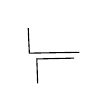
\begin{tikzpicture}[x=1em,y=1em,baseline]\draw (0,1.6)--(.04,.7)--(1.85,.73); \draw (1.66,.52)--(.31,.49)--(.34,-.39);\end{tikzpicture}} Le théorème est conséquence \deleted{\unsure{du théo|du théo.}}\inserted{de} cet \unsure{én$^{\mathrm{t}}$|én$^{\mathrm{cé}}$|est} équivalent

\unsure{à)|a')|a)|:)}

\uline{Théorème} $1'$ Soit $C$ une partie de $E$. Pour que $C$ soit convexe et fermé, il f. et s. que $C$ soit intersection de demi-espaces fermés.

Résulte du

\uline{Théorème $1''$} (Hahn-Banach) Soit $\deleted{\unsure{C}}U$ une partie \uline{convexe ouverte} de l'espace vectoriel \inserted{réel} $E$ de dim finie, $F\subsetneq E$ un sous-espace vectoriel de $E$ tel que $F\cap\deleted{\unsure{C}}U=\varnothing$, alors $\exists$ hyperplan $H$ de $E$ contenant $F$, tel que $H\cap U=\varnothing$.

\scanpage{8}
% archive sheet number: 7

\deleted{\unsure{Résulte|Résultats}} \uline{Dém} \unsure{En effet} : remplacer $U$ par $\bigcup_{\lambda>0}\lambda U$, OPS $U$ un \uline{cône} (\deleted{\unsure{y}} i.e. stable par multiplication par $\lambda>0$) Il suffit de prouver que si

$F$ n'est pas un hyperplan, $\exists F'\supset F$, $F$ de codim $1$ dans $F'$ i.e. $\dim F'=\dim F+1$. OPS $\dim E=\dim F+\unsure{2|1}$.

\unsure{En effet} : passant au quotient par $F$, on est ramené au cas $\dim E=2$, $F=0$. OPS $U\ne\varnothing$

On montre alors que ou bien $U$ est un demi-espace ouvert, ou bien $\exists$ base $e_1,e_2$ tel que $U=\{\lambda_1 e_1+\lambda_2 e_2\mid\lambda_1,\lambda_2>0\}$

\figure{\begin{tikzpicture}[x=1cm,y=1cm,line cap=round]
\fill (0,0) circle (1.6pt);
\draw[->] (0.07,-0.02) .. controls (0.48,-0.08) and (1.18,0.14) .. (1.86,0.07);
\draw[->] (-0.03,0.24) -- (-0.33,1.45);
\draw (-0.33,1.45) -- (-0.48,2.02);
\end{tikzpicture}}

Dans les deux cas on gagne ....

\figure{\begin{tikzpicture}\draw (0,1.55) -- (1.6,0);\end{tikzpicture}}

$\ast$ \uline{Secteurs polyédraux}

\uline{Prop} Soit $C$ partie de $E$ (espace affine de dim finie) Conditions équivalentes

a) $C$ intersection finie de demi-espaces fermés

b) $C$ enveloppe convexe fermée d'un nb fini de pts et de demi-droites fermées. (qu'on peut supposer \deleted{\unsure{partir|partant}}\inserted{\unsure{avoir|ayant|issues}} pour origine un pt $x\in C$ donné à l'avance ...)

b') (Si $C$ compact) $C$ est un polyèdre convexe

\scanpage{9}
% archive sheet number: 8

\uline{Dém} Si $C=\varnothing$ les deux conditions sont satisfaites. Donc OPS $C\ne\varnothing$. \deleted{Soit $x\in C$, on le prend comme origine.} OPS $C$ convexe fermé,

\deleted{donc $C=\unsure{C'{}^\circ|C^{\circ\circ}}$, $C'=C^\circ$} \inserted{et OPS $C$ engendre l'esp \deleted{\unsure{vect}}\inserted{affine} $E$} (car on voit que les deux conditions \inserted{sur $C$} ne changent pas si on remplace $E$ par $E_C$).

Soit $x\in\mathring C$, on le prend comme origine. On aura $C=C'{}^{\circ}$, \inserted{où} $C'=C^\circ$. \unsure{Donc|D'où} $C'$ est compact.

\deleted{$\unsure{A\subset C|A^\circ\subset C}$}

\deleted{b) $\Longrightarrow$ a) Car $\unsure{C'|C''}$ \deleted{\unsure{sera}} étant \deleted{intersection} \inserted{enveloppe} convexe, fermée d'un \unsure{pts|nb|ens.} fini de pts et \deleted{finie d'hyperplans fermés, $C'$ sera l'enveloppe} de demi-droites fermées, $C'$ sera \unsure{env.} fermée d'un nb fini de pts (y inclus \unsure{$0$})}

\deleted{b) $\Longrightarrow$ a) \inserted{Comme on a b} $C'$ sera \deleted{enveloppe convexe (fermée)} intersection \deleted{d'un nb} finie \deleted{de pts (y compris $0$). Si $C$ est compact,} on sait en déduire que $C'$ est intersection d'un nb fini de demi-espaces fermés, on aura gagné par polarité.}

b) $\Rightarrow$ a) Si b) est vrai pour $C$, alors par polarité - $C'$ \deleted{est} int. finie de $1/2$ espaces fermés, donc (lemme ci-dessous) étant compact, c'est un polyèdre convexe, i.e. env. conv. \deleted{finie de}\inserted{d'une} partie finie de $E'$, d'où a) par polarité.

\scanpage{10}
% archive sheet number: 9

a) $\Longrightarrow$ b) On voit \inserted{par polarité} que $C'$ est \deleted{\unsure{réunion}}\inserted{env.} conv. fermée d'un nb fini de pts, \deleted{et de demi-droites d'origine $0$} donc d'après ce qui précède il \deleted{donc $C'$ est \unsure{enveloppé de|enveloppe de}} est intersection finie de demi-espaces \deleted{\unsure{finie et}} fermés donc par polarité on trouve b) pour $E$, sous forme précise.

\figure{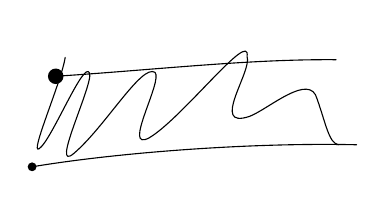
\begin{tikzpicture}[x=1cm,y=1cm,line cap=round,line join=round]
\draw (0.3,1.15) .. controls (1.55,1.23) and (2.75,1.37) .. (3.86,1.36);
\draw (0,0) .. controls (1.14,0.19) and (2.84,0.31) .. (4.12,0.28);
\fill (0.3,1.15) circle (2.8pt); \fill (0,0) circle (1.6pt);
\draw (0.42,1.39) .. controls (0.38,1.10) and (-0.04,0.14) .. (0.09,0.23)
.. controls (0.25,0.34) and (0.66,1.37) .. (0.73,1.19)
.. controls (0.78,1.05) and (0.22,-0.09) .. (0.53,0.17)
.. controls (0.93,0.51) and (1.39,1.31) .. (1.56,1.20)
.. controls (1.67,1.10) and (1.13,0.17) .. (1.49,0.37)
.. controls (1.91,0.62) and (2.78,1.76) .. (2.73,1.40)
.. controls (2.80,1.22) and (2.25,0.47) .. (2.76,0.64)
.. controls (3.00,0.73) and (3.53,1.21) .. (3.62,0.86)
.. controls (3.73,0.55) and (3.77,0.30) .. (3.89,0.28);
\end{tikzpicture}}

\margin{\begin{tikzpicture}[x=1em,y=1em]\draw (0,1.4)--(.04,0);\end{tikzpicture}} \uline{Lemme} Soit $C$ \inserted{compact} int. finie de demi-espaces fermés. Alors \deleted{$C$ est un polyèdre convexe.} \inserted{l'ens des pts extrémaux de $C$ est fini (donc $C$ est un polyèdre convexe s'il est cpct).}

\deleted{En d'autres termes, $C$ n'a qu'un nb fini de pts extrémaux.}

Récurrence \deleted{sur $\unsure{\nu=n+\dim E}$, \unsure{où} \illegible{1}} \inserted{$\dim E$ (trivial si $\dim E=0$) puis sur le} nb $\unsure{\nu|v}$ de demi-espaces qui \unsure{rentrent|entrent}. Trivial si $\nu=0,1$

\deleted{(et $=$ : \unsure{donc si} $n=0$, et $=$ si $n=1$ \unsure{$\}$} alors si $\nu=1$) Supposons}

On est ramené au cas d'un convexe $C_1$ n'ayant qu'un nb fini de pts extrémaux, et où on a

\[
 C=C_1\cap H\qquad
 \begin{aligned}
 &\text{($H$ demi-espace fermé,}\\
 &\text{limité par l'hyperplan}\\
 &H_0)
 \end{aligned}
\]

Soit $x\in C$. \deleted{un pt extrémal.} Si $x\notin H_0$, alors $x$ est pt extrémal de $C$ ssi il est pt extrémal de $C_1$. Si $x\in H_0$, \deleted{et si} $x$ \inserted{est} pt extrémal de $C$, ssi il est pt extrémal de \deleted{$C_1$, \unsure{de}} $H_0\cap C$. On gagne.

\scanpage{11}
% archive sheet number: 10

\uline{Définition} Secteur polyédral : partie satisfaisant aux conditions équivalentes précédentes.

\uline{Prop} $E,E'$ vectoriels de dim finie en dualité. Alors par $A\unsure{\vdash|\mapsto}A^{\unsure{\circ|0}}$, $A'\vdash A'{}^\circ$ on trouve des correspondances $1$-$1$ inverses l'une de l'autre entre secteurs polyédraux de $E$ \unsure{passant|contenant} \deleted{\unsure{par}} \unsure{l'origine|d'origine}, et sect. \unsure{pol.} de $E'$ \unsure{contnt|contenant} l'origine.

\textcircled{\unsure{8|$\ast$}} Polarité et facettes

$E,E'$ Vectoriels de dim finie en dualité. Correspondance biunivoque entre sous-espaces affines $F$ de $E$ ne contenant pas l'origine, et sous espaces \inserted{affines} $F'$ de $E'$ ne contenant pas l'origine, on a

\margin{Notation $F^{\unsure{\vee|\circ|0}}$,}

\[
 \dim F+\dim F^\vee=n-1\qquad(n=\dim E=\dim E')
\]

Correspondance caractérisée par les propriétés a) \unsure{Renverser|Renverse} la relation d'inclusion

b) \unsure{À|$A'$} $x\in E-\{0\}$ correspond $\{x\}^\vee=H(x)^{\bullet}=(\{x\}^{\circ})^\bullet$

\scanpage{12}
% archive sheet number: 11

\uline{Terminologie} Variété d'appui d'un convexe $C$ $=$ variété affine de la forme $E_F$. Les variétés d'appui sont en corr. $\unsure{1\text{-}2|1\text{-}1}$ avec les facettes, relation d'ordre la relation d'inclusion

\margin{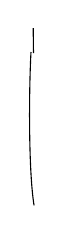
\begin{tikzpicture}[x=1em,y=1em]\draw (.15,6.4)--(.16,5.5); \draw (.07,5.54) .. controls (0,4.3) and (-.03,1.3) .. (.18,0);\end{tikzpicture}} \uline{Th} Soit $C,C'$ deux secteurs polyédraux polaires l'un de l'autre de $E,E'$ resp$^{\mathrm t}$. Alors il existe une unique \deleted{\unsure{corresp}} application $\unsure{\varphi|\phi}$ de l'ens des facettes $F$ de $C$ telles que $0\notin\overline F$ (i.e. $0\in E_F$) vers l'ens des facettes $F'$ de $C'$ telles que $0\notin\overline{F'}$ (i.e. $0'\in E_{F'}$), caractérisée par la propriété que \deleted{si $F'=\varphi(F)$,} \deleted{\unsure{on a} $E$}

\[
 E_{\varphi(F)=F'}=(E_F)^{\unsure{\vee|\circ|0}}
\]

Cette application est bijective, et renverse la relation d'ordre entre facettes

\uline{Cor. 1} L'ens des facettes d'un secteur polyédral est fini (prendre l'origine \uline{intérieure} au secteur polyédral, et appliquer dualité)

\uline{Cor 2} Supposons $C,C'$ cpct \deleted{\unsure{resp.}} i.e. \deleted{$\unsure{\in|C|E}$} $0_E,0_{E'}$ \unsure{intérieurs} à $C,C'$ resp$^{\mathrm t}$, i.e. $C,C'$ des polyèdres. Alors $\varphi:\unsure{\operatorname{Facl}|\operatorname{Fac}}(C)\simeq\unsure{\operatorname{Facl}|\operatorname{Fac}}(C')$

\scanpage{13}
% archive sheet number: 12

(antiisomorphisme d'ens ordonnés).

\uline{Corollaire 3} Soit $\Phi$ un polyèdre combinatoire strict. Alors

a) $\Phi^{\unsure{\circ|o}}$ est un pol. combinatoire strict

b) Si $x,y\in\Phi$, avec $x\leq y$, alors l'ens. ordonné $\Phi_{xy}=\deleted{\unsure{f\ \colon\ x\leq z}}\{z\in\Phi\mid x\unsure{<|\leq}z\leq y\}$ est un polyèdre combinatoire strict.

\uline{Dém} a) Résulte du Cor. 2. On sait que $\Phi_{0,\unsure{x|y}}$ \margin{\begin{tikzpicture}[x=1em,y=1em]\draw[->] (0,.7) .. controls (-.1,0) and (.15,.12) .. (.55,.12);\end{tikzpicture} plus petit \unsure{élém|élém$^{\mathrm t}$|élt}} est un polyèdre combinatoire strict, donc par dualité aussi $\Phi_{x,1}$ \margin{\begin{tikzpicture}[x=1em,y=1em]\draw[->] (0,.35)--(.05,.05)--(.95,.08);\end{tikzpicture} pls grd él} 

$=(\Phi^{\circ}_{0,x})^\circ$. Appliquant ce dernier résultat à $x\in\Phi_{\unsure{0},y}$, on trouve que $\Phi_{xy}$ est un polyèdre combinatoire \unsure{stricte|strict}.

\deleted{\uline{\unsure{Cor 4|Cor. 4}} Soit \unsure{$x,y$} deux facettes}

\deleted{\uline{Cor. 4} \deleted{Soit $F$ une facette d'un p.} $C$ un polyèdre convexe. $F$ une facette \unsure{du dit|dudit}, $i$ \inserted{$\in\mathbb Z$} tel que $-1\leq i\leq d=\dim F$. Alors $\exists$ facette \deleted{de} $F'$ \unsure{incidente} à $F$ telle que $\dim F'=\unsure{i|.|{}}$}

\scanpage{14}
% archive sheet number: 13

\deleted{Si $d=-1$ \deleted{ou $d=0$,}\inserted{ou $d=0$} c'est évident. Supposons $d\geq 1$, i.e. $F\ne\varnothing$, on sait que $F$ est l'enveloppe convexe de l'ens de ses pts extrémaux, donc $\exists F'\in\operatorname{Fac}(C)$ \unsure{un|avec} \unsure{dim} $F'=0$, et $F'\deleted{\unsure{\subset|<}}\inserted{\leq}F$, \deleted{\unsure{donc}}\inserted{en fait} $F'<F$.}

$\ast$ \uline{Application à la fonction dimension}

\margin{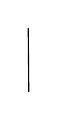
\begin{tikzpicture}[x=1em,y=1em]\draw (0,2.3)--(.02,0);\end{tikzpicture}} \uline{Cor. 4} Soit $C$ un polyèdre convexe, $F_1,\deleted{\unsure{C_2}}F_2\in\operatorname{Fac}(C)$ avec $F_1<F_2$. Pour que $F_2$ soit un \uline{successeur} de $F_1$ (i.e qu'il n'existe pas $F$ tel que $F_1<F<F_2$) il f et s qu'on ait

\[
 \dim F_2=\dim F_1+1
\]

Comme $\dim F$ est fonction \uline{\unsure{strictt|stricte}} croissante sur $\operatorname{Fac}(C)$, la suffisance est claire. Pour la nécessité, \deleted{\unsure{c'est clair si} $\dim F$ \unsure{par}} OPS \inserted{d'abord} $F_2=\deleted{\unsure{F_C|\mathring C}}1$ (plus grande facette), \deleted{et $F_2$} puis en passant au polaire (échange les rôles de $F_1$ et $F_2$) que $F_1=\deleted{\unsure{\varnothing}}0$ (plus petite facette), et à nouveau $F_2=1$. Donc

l'assertion devient maintenant : Pour que il n'existe aucune facette \deleted{\illegible{1}} distincte de $\mathring C$ et de la facette vide, il f et s que $\dim C\unsure{\leq|=}0$ ou $-1$ i.e. que $C$ \inserted{vide ou} réduit à un pt. \deleted{\unsure{car}} (Sinon, en effet, on prend point extrémal !) 

\uline{Cor. 5} La fonction \inserted{$d:F\unsure{\mapsto|\vdash}$} $\dim F$ sur $\operatorname{Fac}(C)$ (du cor. 4) est caractérisée par les conditions

a) $d(F_{\unsure{2|1}})=d(F_1)+1$ si $F_2$ est un successeur de $F_1$

b) $d(\varnothing)=-1$ \margin{\begin{tikzpicture}[x=1em,y=1em]\draw[->] (0,.35) .. controls (0,.02) and (.28,.08) .. (.75,.09);\end{tikzpicture} plus petit él.} De plus $d$ est str. \unsure{croissante|croissant}
